%% abtex2-modelo-livro.tex, v<VERSION> ycherem
%% Copyright 2012-2013 by abnTeX2 group at http://abntex2.googlecode.com/
%%
%% This work may be distributed and/or modified under the
%% conditions of the LaTeX Project Public License, either version 1.3
%% of this license or (at your option) any later version.
%% The latest version of this license is in
%%   http://www.latex-project.org/lppl.txt
%% and version 1.3 or later is part of all distributions of LaTeX
%% version 2005/12/01 or later.
%%
%% This work has the LPPL maintenance status `maintained'.
%%
%% Further information is available on 
%% http://abntex2.googlecode.com/
%%
%% This work consists of the files
%% abntex2-modelo-livro.tex, abntex2-modelo-references.bib,   
%% abntex2-modelo-livro-pintassilgo.jpg,
%% abntex2-modelo-livro-saira-amarela.jpg,
%% abntex2-modelo-livro-bandeirinha.jpg
%%

\documentclass[
	% -- opções da classe memoir --
	10pt,				% tamanho da fonte
	openright,			% capítulos começam em pág ímpar (insere página vazia caso preciso)
	twoside,			% para impressão em verso e anverso. Oposto a oneside
	a5paper,			% tamanho do papel. 
	% -- opções da classe abntex2 --
	%chapter=TITLE,		% títulos de capítulos convertidos em letras maiúsculas
	%section=TITLE,		% títulos de seções convertidos em letras maiúsculas
	%subsection=TITLE,	% títulos de subseções convertidos em letras maiúsculas
	%subsubsection=TITLE,% títulos de subsubseções convertidos em letras maiúsculas
	% -- opções do pacote babel --
	english,			% idioma adicional para hifenização
	french,				% idioma adicional para hifenização
	spanish,			% idioma adicional para hifenização
	brazil,				% o último idioma é o principal do documento
]{abntex2}

% compilação de fontes

\usepackage{ifxetex}
\ifxetex
  % % se for utilizar as fontes do sistema: **escolha sua fonte**
  \usepackage{polyglossia}
  \setmainlanguage{brazil}
  \setotherlanguages{french,english,spanish,german,italian}
  \usepackage{fontspec}
  \defaultfontfeatures{Ligatures=TeX}
  % comandos de fontes
  \setmainfont[Numbers=OldStyle]{Minion Pro} %fonte principal (serifada)
  \setsansfont[Scale=0.9]{Myriad Pro} %fonte sem serifas
  \setmonofont[Scale=MatchLowercase]{Consolas} % fonte monoespaçada
\else
  % % se for utilizar pdflatex
  \usepackage[utf8]{inputenc}
  \usepackage[T1]{fontenc}
  \usepackage{fourier}
  \usepackage[defaultsans]{droidsans} %fonte droid sans como default sans, ao invés de CM Sans.
  \usepackage[scaled=0.9]{inconsolata} %fonte inconsolata para códigos
  \usepackage[defaultmono,scale=0.8]{droidmono} %fonte droid mono para códigos
\fi

%% Observação: o pacote polyglossia pode apresentar erro ao ser utilizado com ifxetex + babel. 
%% Se isso acontecer, atualize o pacote para a versão mais recente ou utilize somente uma das sequências (pdflatex ou xelatex), comentando ou apagando a outra.

\usepackage{microtype} 				% para melhorias de justificação
\usepackage[dvipsnames]{xcolor} 	% para cores
\usepackage{graphicx} 				% para imagens
\usepackage{booktabs,tabularx,rotating}% para tabelas
\usepackage{mdframed} 				% para caixas de texto como na CIP do verso do título
\usepackage{multicol}				% tabelas com colunas mescladas
\usepackage{lettrine}				% letras capitulares
\usepackage{xspace} 				% para nao precisar de espaços com {} depois de comandos
									% como \LaTeX e abreviações criadas pelo usuário
\usepackage{lipsum} 				% para texto de preenchimento de exemplo
\usepackage{leading}				% espaçamento entrelinhas (leading)
\leading{13pt}

% ---
% Pacotes de citações
% ---
\usepackage[brazilian,hyperpageref]{backref}	 % Paginas com as citações na bibl
\usepackage[alf]{abntex2cite}	% Citações padrão ABNT

% ---
% Configurações do pacote backref
% Usado sem a opção hyperpageref de backref
\renewcommand{\backrefpagesname}{Citado na(s) página(s):~}
% Texto padrão antes do número das páginas
\renewcommand{\backref}{}
% Define os textos da citação
\renewcommand*{\backrefalt}[4]{
	\ifcase #1 %
		Nenhuma citação no texto.%
	\or
		Citado na página #2.%
	\else
		Citado #1 vezes nas páginas #2.%
	\fi}%
% ---

% ---
% Informações do documento
% ---
\titulo{Exemplo de livro produzido com \abnTeX}
\autor{Fulano de Tal}
\data{2013}
\preambulo{Breve sinopse do livro}
\local{São Paulo}
\instituicao{Publicações Acadêmicas Ltda.\\ \abnTeX\ v<VERSION>}

% alterando o aspecto da cor azul
\definecolor{blue}{RGB}{41,5,195}

% informações do PDF
\makeatletter
\hypersetup{
     	%pagebackref=true,
		pdftitle={\@title}, 
		pdfauthor={\@author},
    	pdfsubject={\imprimirpreambulo},
	    pdfcreator={LaTeX with abnTeX2},
		pdfkeywords={abnt}{latex}{abntex}{abntex2}{livro}, 
		colorlinks=true,       		% false: boxed links; true: colored links
    	linkcolor=blue,          	% color of internal links
    	citecolor=blue,        		% color of links to bibliography
    	filecolor=magenta,      		% color of file links
		urlcolor=blue,
		bookmarksdepth=4
}
\makeatother
% ---


% ---
% Estilo de capítulos
%
% \chapterstyle{pedersen} 
% \chapterstyle{lyhne} 
%\chapterstyle{madsen} 
\chapterstyle{veelo} 
%
% Veja outros estilos em:
% http://www.tex.ac.uk/tex-archive/info/MemoirChapStyles/MemoirChapStyles.pdf
% ---

% para cabeçalhos sem estar em maiúsculas
%\nouppercaseheads 

% -----
% Declarações de cabecalhos 
% -----
% Cabecalho padrao
\makepagestyle{abntbookheadings}
\makeevenhead{abntbookheadings}{\ABNTEXfontereduzida\thepage}{}{\ABNTEXfontereduzida\textit\leftmark}
\makeoddhead{abntbookheadings}{\ABNTEXfontereduzida\textit\rightmark}{}{\ABNTEXfontereduzida\thepage}
\makeheadrule{abntbookheadings}{\textwidth}{\normalrulethickness}

% Cabecalho do inicio do capitulo
\makepagestyle{abntbookchapfirst}
\makeoddhead{abntbookchapfirst}{}{}{}

% Configura layout para elementos textuais
\renewcommand{\textual}{%
  \pagestyle{abntbookheadings}%
  \aliaspagestyle{chapter}{abntbookchapfirst}% customizing chapter pagestyle
  \nouppercaseheads%
  \bookmarksetup{startatroot}% 
}
% ---

% ---
% Espaçamentos entre linhas e parágrafos
% ---
% O tamanho do parágrafo é dado por (exemplo):
%\setlength{\parindent}{1.3cm}
%% Não recomendado mudar.
 
% Controle do espaçamento entre um parágrafo e outro:
%\setlength{\parskip}{0.2cm}  % tente também \onelineskip
%% Não recomendado mudar.

% Margens do documento 
%% (margens do abntex2 não combinam nem com A5 nem com estilos de capítulo da
% classe memoir.)
\setlrmarginsandblock{2.5cm}{3.5cm}{*}
\setulmarginsandblock{2.5cm}{3.5cm}{*}
\checkandfixthelayout
% ---


% ---
% Início do documento
% ---
\begin{document}
\frenchspacing

\frontmatter

% ---
% Capa principal
% ---
\begin{titlingpage}
\phantom{xxx}
\vspace{0.5cm}
\huge
\raggedright
\imprimirautor\\
\vspace{2.5cm}
\Huge 
{\raggedleft
\textit{\textcolor{blue}{\imprimirtitulo}}\\[1cm]
}
\centering 
%  %este é um símbolo que só aparecerá com a fonte Minion.
\vfill
\Large
% %este é um símbolo que só aparecerá com a fonte Minion.
\imprimirinstituicao
\end{titlingpage}
% ---

% ---
% Contra-capa
% ---
\begin{titlingpage}

\phantom{xxx}
\vspace{0.5cm}
\huge
\raggedright
\imprimirautor\\
\vspace{2.5cm}
\Huge 
{\raggedleft
\textit{\textcolor{blue}{\imprimirtitulo}}\\[1cm]
}
\centering 
% %este é um símbolo que só aparecerá com a fonte Minion.
\vfill
\Large
% %este é um símbolo que só aparecerá com a fonte Minion.
\imprimirinstituicao
% ---

% ---
% Verso da contra-capa
% ---
\clearpage
\ABNTEXfontereduzida
%\raggedright
© 2013 \imprimirautor \space \& \imprimirinstituicao
%este é só um exemplo de copyright.

Qualquer parte desta publicação pode ser reproduzida, desde que citada a fonte.

\vspace*{\fill}

\begin{center}
Dados Internacionais de Catalogação na Publicação (\textsc{cip})
Câmara Brasileira do Livro, \textsc{sp}, Brasil
\end{center}

\begin{mdframed}
\noindent Tal, Fulano de.

\imprimirtitulo. / \imprimirautor. -- \imprimirlocal: \imprimirinstituicao
Ltda., 2013.

\medskip

Bibliografia.

ISBN XXXX-XXXX-XX.

\medskip

1. Programas de computador. 2. Tipografia. 3. Latex. 4. Normas ABNT.

\end{mdframed}

\end{titlingpage}
% ---

% ---
% Agradecimentos
% ---
\begin{agradecimentos}
Este trabalho é fruto da ação de membros da comunidade \abnTeX. Porém, ele não
seria real se não fosse o trabalho e a dedicação incondicional de Youssef
Cherem, a quem o responsável atual pelo projeto, Lauro César Araujo, agradece
incondicionalmente.
\end{agradecimentos}
% ---

% ---
% inserir lista de ilustrações
% ---
\pdfbookmark[0]{\listfigurename}{lof}
\listoffigures*
\cleardoublepage

% ---
% inserir lista de tabelas
% ---
\pdfbookmark[0]{\listtablename}{lot}
\listoftables*
\cleardoublepage
% ---

% ---
% inserir o sumario
% ---
\pdfbookmark[0]{\contentsname}{toc}
\tableofcontents*
\cleardoublepage
% ---

% ------------------------------------------------------------
% Início da parte textual
% ------------------------------------------------------------
%\textual
\mainmatter
% ------------------------------------------------------------

% ------------------------------------------------------------
\chapter*[Introdução]{Introdução}
\addcontentsline{toc}{chapter}{Introdução}
% ------------------------------------------------------------

\lettrine[nindent=0.35em,lhang=0.40,loversize=0.3]{E}{ste documento} faz parte
do projeto \abnTeX\footnote{\url{http://abntex2.googlecode.com/}}, e destina-se
a servir de modelo para composição e diagramação de livros e folhetos em
\LaTeX em conformidade com a norma ABNT NBR 6029:2006 \emph{Informação e
documentação - Livros e folhetos - Apresentação}. 

Em geral, qualquer classe do \LaTeX\ que contemple o formato de livros poderia
ser utilizada (como \textsf{book}, \textsf{memoir} e \textsf{scrbook}, entre
outras). A formatação de geral dos capítulos, margens, tamanho de página,
fontes, etc., segundo a norma ABNT em questão, pode ser modificada pelo usuário
à vontade.

Porém, este modelo foi composto com a classe \textsf{abntex2.cls} com o intuito
de estimular que autores de teses e dissertações convertam e publiquem seus
trabalhos em forma de livro. 

Essencialmente, este modelo é idêntico aos demais modelos distribuídos com o
\abnTeX. Porém, este documento exemplifica como customizar a formatação final do
documento para que ele fique adequado aos padrões de publicação de livros.
Observe que há vários comentários no código-fonte do arquivo, de modo a
facilitar ao máximo as customizações. Consulte o portal do projeto para obter
acesso aos manuais, wiki, e grupos de discussões do \abnTeX.

Em linhas gerais, a norma ABNT NBR 6029:2006 não estabelece parâmetros tão
rígidos quanto a ABNT NBR 14724:2011, para trabalhos acadêmicos, e segue, de
certa forma, o design usual de livros\footnote{Para facilitação da compreensão
de termos técnicos, ver a Tabela \ref{vocabulario-texto} com alguns termos do
design de livros.}.

Desta forma, temos:

\begin{description}
\item[parte pré-textual] Composta por: falsa folha de rosto, folha de rosto,
colofão (opcional na parte pós-textual), sumário (conteúdo),
a\-gra\-de\-ci\-men\-tos (acknowledgments), dedicatória, epígrafe;
\item[folha de rosto] Como diz o nome em inglês (\textit{title page}) a ``folha
de rosto'' é a \textit{página do título}. No verso da folha de rosto, costuma-se
incluir os dados sobre a obra e a edição, catalogação, editora, direitos
autorais e de reprodução, etc;
\item [parte pós-textual] Composta por epílogo, posfácio, apêndice, glossário,
bibliografia, índice remissivo (inglês: \textit{index}), colofão, etc;

\end{description}

Este documento deve ser utilizado como complemento dos manuais do \abnTeX\ 
\cite{abntex2classe,abntex2cite,abntex2cite-alf} e da classe \textsf{memoir}
\cite{memoir}. 

  
% ------------------------------------------------------------
\chapter{Um exemplo de capítulo}
% ------------------------------------------------------------

\lipsum[1-10]

% ------------------------------------------------------------
\chapter{Exemplos de imagens}
% ------------------------------------------------------------

\lipsum[1]

\begin{figure}
\centering
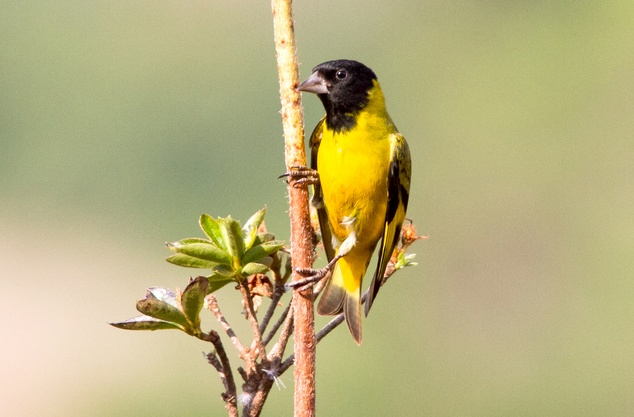
\includegraphics[width=0.6\linewidth]{abntex2-modelo-livro-pintassilgo}
\caption{Pintassilgo (\textit{Carduelis magellanicus}).}
\label{fig:pintassilgo}
\end{figure}

\lipsum[6]

\begin{figure}
\centering
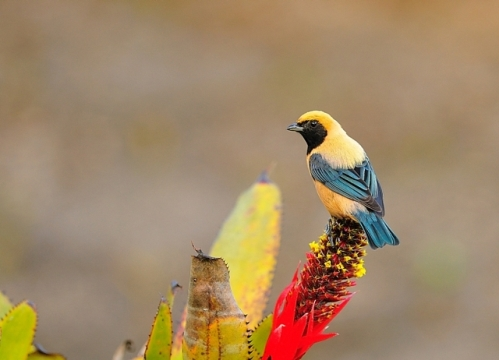
\includegraphics[width=0.6\linewidth]{abntex2-modelo-livro-saira-amarela}
\caption{Saíra-amarela (\textit{Tangara cayana}).}
\label{fig:saira-amarela}
\end{figure}

\begin{figure}
\centering
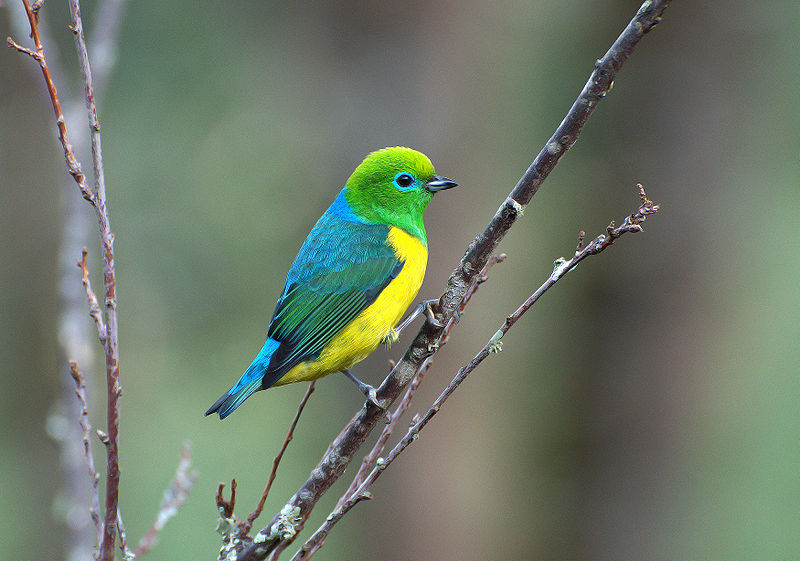
\includegraphics[width=0.6\linewidth]{abntex2-modelo-livro-bandeirinha}
\caption{Bandeirinha (\textit{Chlorophonia cyanea}).}
\label{fig:bandeirinha}
\end{figure}


\lipsum[7]

% ------------------------------------------------------------
\chapter{Exemplos de tabela}
% ------------------------------------------------------------

\section{Uma seção}

\lipsum[8]

\begin{table}
\caption{Pequeno vocabulário de design de livros\label{vocabulario-texto}}
\ABNTEXfontereduzida
\begin{tabular}{p{4cm}p{4cm}}
\toprule
\textit{Termo em inglês} & \textit{Termo em português}\\
\midrule
\ABNTEXfontereduzida
title page & folha de rosto.\\

cover & capa\\

back cover & quarta capa ou contra-capa ou verso da capa\\

bastard title ou half title & falsa folha de rosto. Tem só o título do livro.\\

table of contents & sumário\\

text block ou book block & miolo\\

print space (alemão: \textit{Satzspiegel}) & mancha gráfica\\

section, gathering, quire (especialmente se não impresso), signature & caderno\\

leaf = folio (latim) & folha, composta de recto (lat.) (anverso/frente) e verso (lat.) (verso). Geralmente o recto é página ímpar, e verso é página par.\\

hardcover & capa dura.\\

endpaper/endsheet & folha de guarda. Folha de papel para prender o miolo do livro na capa dura.\\

dust jacket, dust cover, book jacket, dust wrapper & sobrecapa. Geralmente de papel, para cobrir capas duras.\\

front matter & parte pré-textual.\\

main matter & parte textual\\

back matter & parte pós-textual. Composta por epílogo, posfácio, apêndice, glossário, bibliografia, índice remissivo (inglês: index), colofão etc.\\

colophon & colofão. Breve descrição sobre aspectos da publicação do livro. \\

running headers & títulos correntes\\

volume & volume. Conjunto de páginas encadernadas.\\

\bottomrule
\end{tabular}
\footnotesize Fontes:\\
\url{http://pt.wikipedia.org/wiki/Design_de_livros}\\
\url{http://en.wikipedia.org/wiki/Book_design}\\
\url{http://static.lexicool.com/dictionary/RX7KW614433.pdf}\\
\end{table}


\begin{table}
\caption{Exemplo de tabela utilizando o pacote \textsf{booktabs}.}
\centering
\begin{tabular}{llr}
\toprule
\multicolumn{2}{c}{Item} \\
\cmidrule(r){1-2}
Animal    & Description & Price (\$) \\
\midrule
Gnat      & per gram    & 13.65      \\
          & each        & 0.01       \\
Gnu       & stuffed     & 92.50      \\
Emu       & stuffed     & 33.33      \\
Armadillo & frozen      & 8.99       \\
\bottomrule
\multicolumn{3}{l}{\ABNTEXfontereduzida Fonte: \url{http://en.wikibooks.org/wiki/LaTeX/Tables}}
\end{tabular}
\end{table}

\lipsum[9]

% ------------------------------------------------------------
\postextual % pós-textual
% ------------------------------------------------------------

% ------------------------------------------------------------
\bibliography{abntex2-modelo-references} % insere o arquivo de bibliografia
% ------------------------------------------------------------

% ------------------------------------------------------------
% Colofão: última página com informações sobre a composição do livro.
\cleardoublepage
\thispagestyle{empty} 

Sinta-se convidado a participar do projeto \abnTeX! Acesse o site do projeto em
\url{http://abntex2.googlecode.com/}. Também fique livre para conhecer, estudar,
alterar e redistribuir o trabalho do ABN\TeX, desde que os arquivos modificados
tenham seus nomes alterados e que os créditos sejam dados aos autores originais,
nos termos da ``The \LaTeX\ Project Public
License''\footnote{\url{http://www.latex-project.org/lppl.txt}}.

Encorajamos que sejam realizadas customizações específicas deste documento.
Porém, recomendamos que ao invés de se alterar diretamente os arquivos do
\abnTeX, distribua-se arquivos com as respectivas customizações.
Isso permite que futuras versões do \abnTeX~não se tornem automaticamente
incompatíveis com as customizações promovidas. Consulte
\citeonline{abntex2-wiki-como-customizar} par mais informações.


% ~\vfill Este texto foi composto em Minion Pro, de Robert Slimbach, e Myriad Pro,
% de Robert Slimbach e Carol Twombly.
~\vfill Este texto foi composto em Utopia, de Robert Slimbach, através do pacote \texttt{fournier}.

\end{document}